\chapter{Experimental evaluation}

\noindent{}TODO: Chapter description and probably add reference to our data repository\footnote{\url{https://github.com/dataspecer/domain-modeling-benchmark}}


\section{Evaluation domains}

To assess the quality of the generators, we used six domains with their domain description and manually created reference domain models.
We used the reference models to evaluate the suggestions generated based on the domain descriptions.
Table \ref{tab:reference-model-size} summarizes the size of these reference models.

\begin{table}[!h]
    \scriptsize
    \centering
    \setlength{\tabcolsep}{0.5em}
    \begin{tabular}{lcccccc}
         & Aircrafts & Papers & Farming & Zoos & Colleges & Vehicles \\
    \toprule
    \addlinespace
         \# classes      & 8  & 7  & 14 & 14 & 63 & 66 \\
         \# attributes   & 10 & 12 & 15 & 26 & 14 & 72 \\
         \# associations & 8  & 9  & 9  & 24 & 67 & 46 \\
    \addlinespace
    \bottomrule
    \addlinespace
    \end{tabular}
    \caption{The size of the reference domain models}
    \label{tab:reference-model-size}
\end{table}


We categorize the domains into two groups.
The first group contains three domains: \emph{aircraft manufacturing}, \emph{conference papers}, and \emph{farming}.
They are characterized by simpler descriptions with a limited scope of concepts.
For each domain, we manually created three semantically equivalent domain descriptions in three different styles.
\emph{Analytical} descriptions are written with analytical precision, describing each concept rigorously, unambiguously, and preferably with a consistent sequence of sentences.
\emph{Eclectic} are written as a collection of less structured knowledge from different stakeholders, each describing the domain from a different point of view.
\emph{Educational} emphasize the most important concepts at the beginning, where only essential aspects are described, followed by adding more details about the concepts later in the description.

Additionally, to assess the quality of our RAG approaches, for each domain description we also manually created corresponding annotated domain description. Each annotated domain description contains tags that for each domain element from the corresponding reference domain model determine the parts that contain information about this domain element. Here is an example of the original domain description and the corresponding annotated domain description from the \emph{farming} domain: \\

\noindent{}Domain description: \textit{A farmer is an individual engaged in agriculture, growing and harvesting crops, and is identified uniquely by a name that is used to refer to the farmer from various documentation, statistical reporting, etc.} \\

\noindent{}Annotated domain description: \textit{\textbf{<farmer>}A farmer is an individual engaged in agriculture, growing and harvesting crops\textbf{</farmer>}, and \textbf{<name>}is identified uniquely by a name that is used to refer to the farmer from various documentation, statistical reporting, etc.\textbf{</name>}}

The corresponding reference model contains the class \textit{farmer} with the attribute \textit{name}. In the annotated text the parts between the opening tag ``\textbf{<farmer>}'' and the closing tag ``\textbf{</farmer>}'' capture the information about the class \textit{farmer}. Similarly, the opening tag ``\textbf{<name>}'' and the closing tag ``\textbf{</name>}'' captures the information about the attribute \textit{name} of the class \textit{farmer}.

The annotated domain description can contain multiple tags with the same name. After an opening tag can follow another opening tag if it has a different name but each tag must be first opened and then closed.


\section{RAG evaluation}
\label{sec:filtering_evaluation}


\subsection{Evaluation methodology}

\subsubsection{Recall}

For a domain element $e$ let $Y_e$ be the set of expected relevant parts that are marked by the tags with the name equal to the $name(e)$. Let $X_e \subseteq Y_e$ be the set of parts from $Y_e$ that the selected RAG approach marked as relevant based on the $name(e)$ if $e$ is a class, otherwise based on the $name(source(e))$. Now when given a domain description with its reference domain model containing a set of domain elements denoted by $E$ where the $E$ can be a set of classes, attributes, or associations. The recall $R$ is computed as:

\[ R = \dfrac{\sum_{e \in E}|Y_e|}{\sum_{e \in E}|X_e|}. \]

\noindent{}where $|Y_e|$ denotes the size of the set $Y_e$ and $|X_e|$ denotes the size of the set $X_e$.


\subsubsection{Precision}

For a class $c$ and domain description $T$ let $Y_{c}$ be the set of expected relevant parts of the class $c$ and of the attributes and associations with the source class equal to $c$. Now let $Z_{c}$ be the set of chunks from the given domain description that the selected RAG approach marked as relevant based on the class $c$. Then the precision $P_{c}$ for the class $c$ and the domain description $T$ is computed as:

\[ P = \dfrac{\sum_{c \in C}|Y_c|}{\sum_{c \in C}|Z_c|}. \]

We do not compute the precision separately for classes, attributes, and associations as the goal of our RAG approach is to find relevant information for a given source class but not to find the information about classes, attributes, and associations separately.


\subsection{Selected models}

For our semantic approach, we use the model \textit{all-MiniLM-L6-v2}\footnote{\url{https://huggingface.co/sentence-transformers/all-MiniLM-L6-v2}}. It is a symmetric embedding model intended for encoding sentences and short paragraphs. As a comparison function, we use cosine-similarity.

Our syntactic approach uses the \textit{MorphoDiTa} tool \cite{Strakova2014} with the \textit{english-morphium-wsj-140407} model for converting English words into lemmas \cite{Straka2014}.


\subsection{Results}

In the section \ref{texts_comparison}, we introduced our semantic and syntactic RAG approach. To comparing these approaches now we also introduce the no-filtering approach where the domain description is not filtered at all. The table \ref{tab:filtering-results} contains the measured results:

\begin{table}[!h]
    \scriptsize
    \centering
    \setlength{\tabcolsep}{0.5em}
    \begin{tabular}{lcccc}

    \toprule
         & Recall classes & Recall attributes & Recall associations & Precision \\
    \toprule
    
    \addlinespace
         no-filtering      & 1.00  & 1.00  & 1.00 & 0.06 \\
    	 syntactic-baseline & 0.87 & 0.79 & 0.84 & 0.55 \\
         syntactic-pronouns-naive & 0.93  & 0.91  & 0.90 & 0.49 \\
         semantic-baseline & 1.00 & 0.98 & 0.98 & 0.10 \\
         semantic-pronouns-naive & 0.99 & 0.96 & 0.97 & 0.10 \\
    \addlinespace
    \bottomrule
    \addlinespace
    \end{tabular}
    \caption{The size of the reference domain models}
    \label{tab:filtering-results}
\end{table}

As expected, the no-filtering approach gets the highest possible recall but also gets the lowest precision.

In the syntactic approach, the naive pronouns detection improves the recall significantly but slightly decreases the precision. This approach can probably offer the best performance as it has the highest precision of all the measured approaches. To improve its relatively low recall, the domain description can be manually pre-processed to remove some problematic constructs such as unexpressed subjects.

The semantic approach almost matches the recall of the no-filtering approach but it has a higher precision. Unexpectedly, the naive pronouns approach slightly decreases the recall while maintaining similar precision.

Overall, when recall is the most important then the no-filtering approach or the semantic approach can be used. On the other hand, when precision is the most important and we do not care about losing some domain element suggestions then the syntactic approach is the most suitable.


\section{Selected LLMs}

Running a LLM requires a lot of resources, therefore frequently using a LLM through some API can cost a lot of money. Thus, we run open-source LLMs locally with LLaMA.cpp server\footnote{\url{https://github.com/ggerganov/llama.cpp/blob/master/examples/server/README.md}}. Our hardware is limited to a single NVIDIA A100 40GB GPU.

\subsection{Limitations}

Because of our hardware limitation we use Mixtral-8x7B\footnote{\url{https://huggingface.co/TheBloke/Mixtral-8x7B-Instruct-v0.1-GGUF/blob/main/mixtral-8x7b-instruct-v0.1.Q5_K_M.gguf}} (medium-sized LLM) \cite{Jiang2024} and Llama-3-70B\footnote{\url{https://huggingface.co/bartowski/Meta-Llama-3-70B-Instruct-GGUF/blob/main/Meta-Llama-3-70B-Instruct-Q5_K_M.gguf}} (relatively large-size LLM) both in quantized variation where on average they have 5 bits per parameter.


\subsection{Mixtral-8x7B}

Mixtral-8x7B has the context window size of 32k tokens and it outperforms or matches ChatGPT-3.5 across many benchmarks \cite{Jiang2024}. This LLM has in total 47B parameters, which are distributed among 8 experts. To achieve faster output generation, for each generated token 2 of the 8 experts are selected. The selection of the experts can be different for each token \cite{Jiang2024}.


\subsection{Llama-3-70B}

Llama-3-70B has an 8k tokens context window size and as of writing this thesis, it is the state-of-the-art LLM at the 70B parameters scale\footnote{\url{https://ai.meta.com/blog/meta-llama-3/}}.


%\section{Limitations}
%
%\begin{itemize}
%\item we used one domain modeling expert for evaluating attributes and associations, we used one student for evaluating classes, and domain elements descriptions
%\item we did preliminary experiments on most of the configurations with one middle sized domain description and then used more domain descriptions for the most promising configurations
%\end{itemize}


\section{Evaluation of generated domain elements}

First, we did a preliminary evaluation where we evaluated many different combinations of prompting techniques, RAG approaches, and LLMs with the domain description \textit{zoological gardens-00}\footnote{\url{https://github.com/dataspecer/domain-modeling-benchmark/blob/main/manual\%20evaluation\%20domains/zoological\%20gardens/domain-description-00.txt}}. Then, we took the combinations with the best results and evaluated them on all our other domain descriptions.


\subsection{Manual assessment of generated suggestions}

Each generated suggestion was manually assessed by a human evaluator who recorded the assessment in the evaluation tables in columns \emph{Matches class}, \emph{Matches attribute}, and \emph{Matches association}.
\emph{Semantic correspondence} between a suggested $X'$ and a reference $X$ $\in$ $M$ is essential for the evaluation.
%The evaluator decides based on the metadata provided about $X'$ and $X$.
If the question \emph{Can we model $X$ also as $X'$?} can be answered positively, $X'$ \emph{semantically corresponds to} $X$.

\begin{table}[!h]
    \scriptsize
    \centering
    \setlength{\tabcolsep}{0.5em}
    \begin{tabular}{lccc}
                     & \emph{Matches class}        & \emph{Matches attribute} & \emph{Matches association} \\
\toprule
\addlinespace
        $gen_c(T)$   & $name(X)$ $\vert$ * $\vert$ & \emph{N/A}  & \emph{N/A} \\
                     & $name(X_1)$;$\ldots$        & \emph{N/A}  & \emph{N/A} \\
\addlinespace
\midrule
\addlinespace
        $gen_a(T,C)$ & $name(D)$ $\vert$ *         & $name(X)$ $\vert$ * $\vert$ & $name(X)$ $\vert$ * $\vert$ \\
        $gen_r(T,C)$ &                             & :$name(X)$ $\vert$ :* $\vert$ & :$name(X)$ $\vert$ :* $\vert$ \\
                     &                             & $name(X_1)$;$\ldots$        & $name(X_1)$;$\ldots$ \\
\addlinespace
\bottomrule
    \end{tabular}
    \caption{Summary of manual evaluation rules}
    \label{tab:manual-assessment-of-suggestions}
\end{table}

To limit subjectivity, we requested that the manual evaluation be carried out according to the rules summarized in Table \ref{tab:manual-assessment-of-suggestions}.
If the class $X'$ suggested by $gen_c(T)$ corresponds to a single class $X$, we record $name(X)$ in \emph{Matches class}.
%The correspondence is determined by whether $name(X')$ refers to the same conceptual entity as $name(X)$.
The assessment considers both the occurrences of $name(X')$ within $T$ and how $X$ is structured within $M$.
If $X'$ does not correspond to any class in $M$, but the evaluator considers it valid from the semantic point of view based on $T$, we record an asterisk (*) in \emph{Matches class}.
%This indicates that according to the judgment of the evaluator, $X'$ represents a concept that could be modeled in $M$ based on its relevance and presence in $T$.
This scenario can arise especially in more complex domains where not all concepts in the domain description are modeled, or a concept can be modeled with an attribute instead of an association and a class.
If $X'$ does not correspond to any single class in $M'$, but its $name(X')$ corresponds to a list of classes $X_1$, $\ldots$, $X_n$ $\in$ $M$, their names are concatenated to $name(X_1)$;$\ldots$;$name(X_n)$ which we record in \emph{Matches classes}.
This corresponds to scenarios where domain models are more coarse-grained.

For a property $X'$ suggested by $gen_a(T,C)$ and $gen_r(T,C)$, we consider similar rules with some differences.
If $X'$ is a suggested attribute, it can also correspond to an association $X$ and vice versa.
This scenario arises in practice, where properties can be modeled as attributes or associations interchangably based on the desired level of semantic and structural detail of the resulting domain model.
Therefore, $name(X)$ is recorded in \emph{Matches attribute} if $X$ is a reference attribute or \emph{Matches association} if $X$ is a reference association.
Moreover, $X'$ must correspond to $X$ also in its source class and, if $X'$ is an association, in its target classes.
$X'$ can be suggested in the reverse direction of $X$.
The asterisk (*) and the lists are used in the same way as for the classes.
In addition, when $X'$ corresponds to an association $X$ then $name(D)$ of the class at the other end of $X$ than the end with $C$ is recorded in \emph{Matches class}.
This corresponds to a scenario where a domain modeler models $D$ not in the step of identifying classes in $T$, but when modeling $X$ starting in $C$.
%In this step, the designer creates $D$ which we record by $name(D)$ in \emph{Matches class}.
When $X'$ corresponds to an association that is not in $M$, the class at the other end of this association is a class $D$ in $M$, which we record again with $name(D)$ in \emph{Matches class}.
Last but not least, it might happen that $X'$ corresponds to $X$ only when the correspondence requirement in the source/target class is relaxed so that the classes at the ends of $X'$ can be subclasses or superclasses of the corresponding classes at the ends of $X$.
In that case, we write a colon(:) followed by $name(X)$ to \emph{Matches attribute} or \emph{Matches class}.
We write a colon followed by an asterisk (:*) if $X'$ makes sense, but should be modeled for a subclass of superclass of $C$.


\subsection{Preliminary evaluation results}

The table \ref{tab:preliminary-mixtral} shows preliminary results for Mixtral-8x7B and the table \ref{tab:preliminary-llama} shows preliminary results for Llama-3-70B.

\begin{table}[!h]
    \scriptsize
    \centering
    \setlength{\tabcolsep}{0.5em}
    \begin{tabular}{lcccccc}
    \toprule
         & & Attributes & & & Associations & \\
     \toprule
         & Recall & Precision & $F_1$ & Recall & Precision & $F_1$ \\
    \toprule
    
    \addlinespace
         baseline-none        & 0.73 & 0.33 & 0.45 & 0.54 & 0.22 & 0.31 \\
    	 baseline-semantic    & 0.73 & 0.35 & 0.47 & 0.75 & 0.27 & 0.40 \\
         baseline-syntactic   & 0.73 & 0.38 & 0.50 & 0.62 & 0.38 & 0.47 \\
         CoT-none             & 0.62 & 0.34 & 0.44 & 0.75 & 0.50 & 0.60 \\
         CoT-semantic         & 0.58 & 0.58 & \textbf{0.58} & 0.67 & 0.39 & 0.49 \\
         CoT-syntactic        & 0.88 & 0.43 & \textbf{0.58} & 0.71 & 0.53 & 0.61 \\
         N-shot-none          & 0.85 & 0.23 & 0.36 & 0.71 & 0.35 & 0.47 \\
         N-shot-semantic      & 0.85 & 0.32 & 0.46 & 0.83 & 0.47 & 0.60 \\
         N-shot-syntactic     & 0.88 & 0.38 & 0.53 & 0.83 & 0.59 & \textbf{0.69} \\
         CoT-N-shot-none      & 0.92 & 0.28 & 0.43 & 0.46 & 0.40 & 0.43 \\
         CoT-N-shot-semantic  & 0.88 & 0.35 & 0.50 & 0.79 & 0.49 & 0.60 \\
         CoT-N-shot-syntactic & 0.92 & 0.37 & 0.53 & 0.79 & 0.53 & 0.63 \\
    \addlinespace
    \bottomrule
    \addlinespace
    \end{tabular}
    \caption{Preliminary evaluation with Mixtral-8x7B strict variation only}
    \label{tab:preliminary-mixtral}
\end{table}


\begin{table}[!h]
    \scriptsize
    \centering
    \setlength{\tabcolsep}{0.5em}
    \begin{tabular}{lcccccc}
    \toprule
         & & Attributes & & & Associations & \\
     \toprule
         & Recall & Precision & $F_1$ & Recall & Precision & $F_1$ \\
    \toprule
    
    \addlinespace
         baseline-none        & 0.96 & 0.80 & \textbf{0.87} & 0.71 & 0.34 & 0.46 \\
    	 baseline-semantic    & 0.88 & 0.64 & 0.74 & 0.79 & 0.49 & 0.60 \\
         baseline-syntactic   & 0.92 & 0.59 & 0.72 & 0.89 & 0.59 & 0.69 \\
         CoT-none             & 0.88 & 0.72 & 0.79 & 0.67 & 0.59 & 0.63 \\
         CoT-semantic         & 0.85 & 0.70 & 0.77 & 0.88 & 0.56 & 0.68 \\
         CoT-syntactic        & 0.92 & 0.52 & 0.66 & 0.88 & 0.54 & 0.67 \\
         N-shot-none          & 0.92 & 0.66 & 0.77 & 0.79 & 0.60 & 0.68 \\
         N-shot-semantic      & 0.88 & 0.57 & 0.69 & 0.88 & 0.56 & 0.68 \\
         N-shot-syntactic     & 0.92 & 0.66 & 0.77 & 0.83 & 0.60 & 0.70 \\
         CoT-N-shot-none      & 0.92 & 0.77 & 0.84 & 0.71 & 0.57 & 0.63 \\
         CoT-N-shot-semantic  & 0.85 & 0.64 & 0.73 & 0.79 & 0.60 & 0.68 \\
         CoT-N-shot-syntactic & 0.92 & 0.66 & 0.77 & 0.83 & 0.67 & \textbf{0.74} \\
    \addlinespace
    \bottomrule
    \addlinespace
    \end{tabular}
    \caption{Preliminary evaluation with Llama-3-70B strict variation only}
    \label{tab:preliminary-llama}
\end{table}

We can see that with Mixtral-8x7B the RAG improves the $F_1$ score for attributes and associations mostly by improving the precision. However, in the case of Llama-3-70B the RAG does not seem to have any noticeable effect probably because the Llama-3-70B is able to find attributes and associations without the domain description filtering when working with the \textit{zoological gardens} domain description which has almost 1000 words.

The baseline prompting technique is the most inconsistent as it has one of the worst $F_1$ scores every time except for the case with Llama-3-70B for attributes where it achieves the best $F_1$ score.

As the CoT-N-shot prompting technique consistently shows good results for generating attributes and associations, we evaluated this technique for all other domain descriptions. \\

\noindent{}TODO: Do preliminary evaluace přidat třídy \\

\noindent{}TODO: Přidat evaluaci pro CoT-N-shot pro všechny popisy domén a odprezentovat to podobně, jako to je v článku


\section{Descriptions evaluation}

For each generated description we evaluated the following tasks:
\begin{itemize}
\item is the description strictly based on the given domain description
\item is the description semantically corresponding to the given domain
\item does the description not contain any useless additional information
\item does the description not miss any useful information \\
\end{itemize}

\noindent{}TODO: Přesněji zadefinovat ten třetí a čtvrtý bod \\

\noindent{}TODO: Napsat, že jako popis domény jsme použili zoological gardens-00

%\begin{figure}[!h]
%    \centering
%    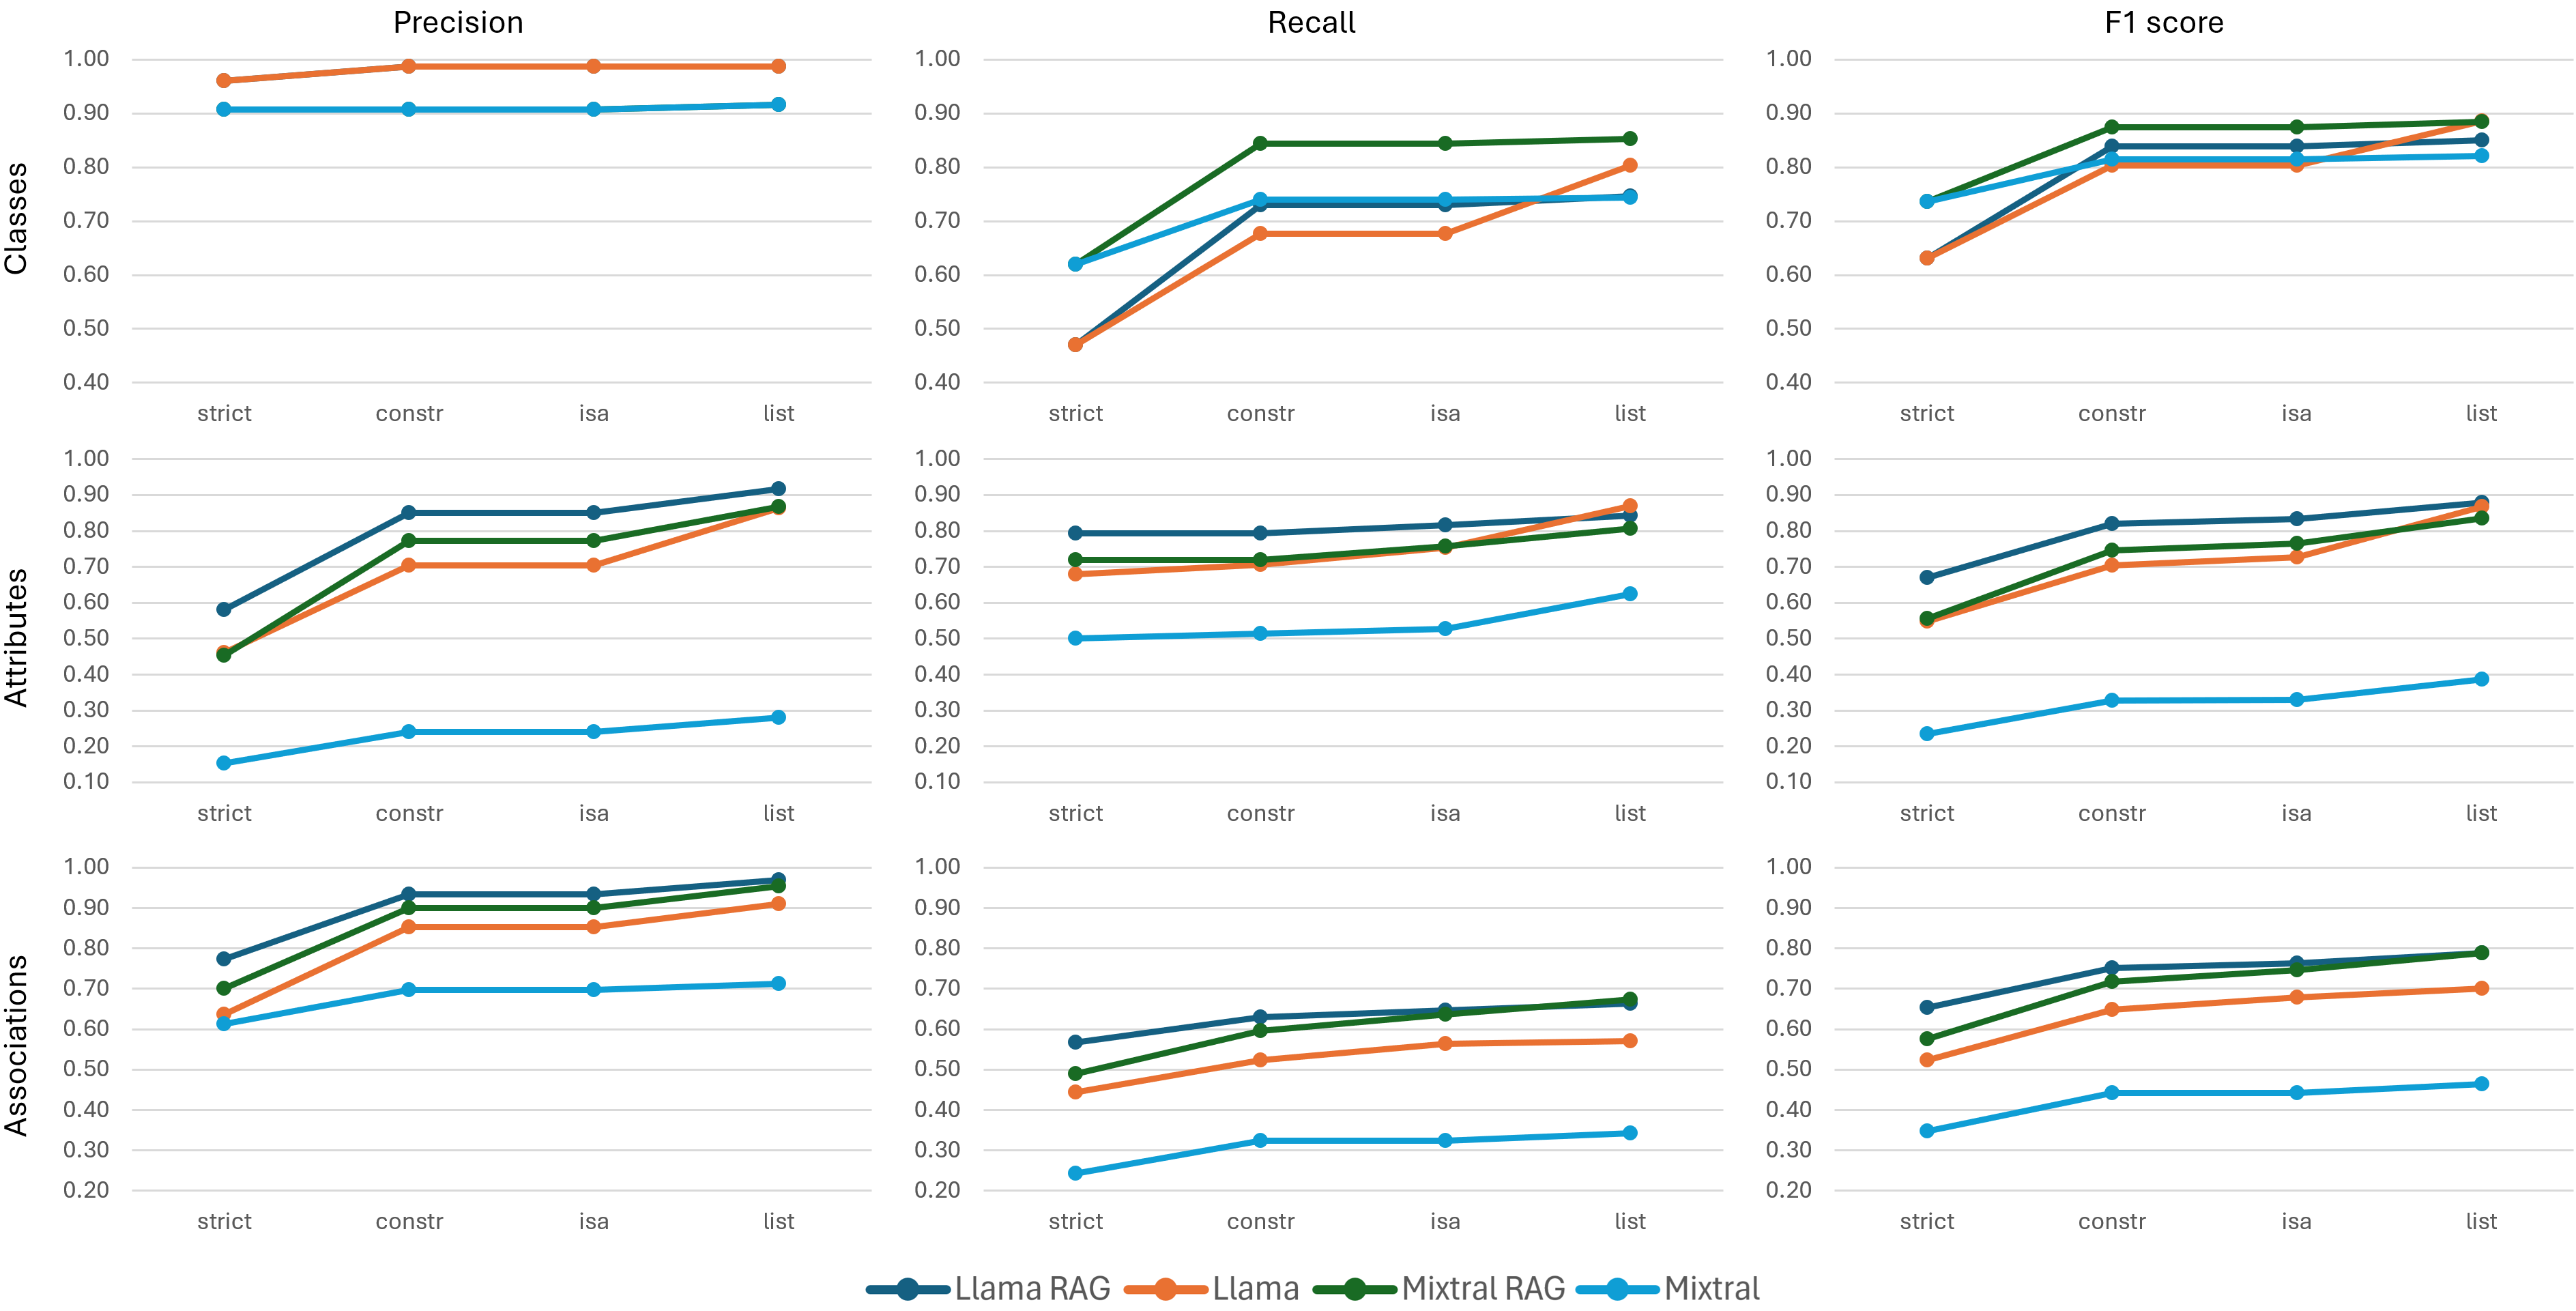
\includegraphics[scale=0.10]{img/evaluation-complex-p-r-f1.png}
%    \caption{\centering Average Precision, recall and $F_1$ scores for the complex domain descriptions at the four levels of matching strictness}
%    \label{fig:evaluation-complex-p-r-f1}
%\end{figure}
%
%\begin{figure}[!h]
%    \centering
%    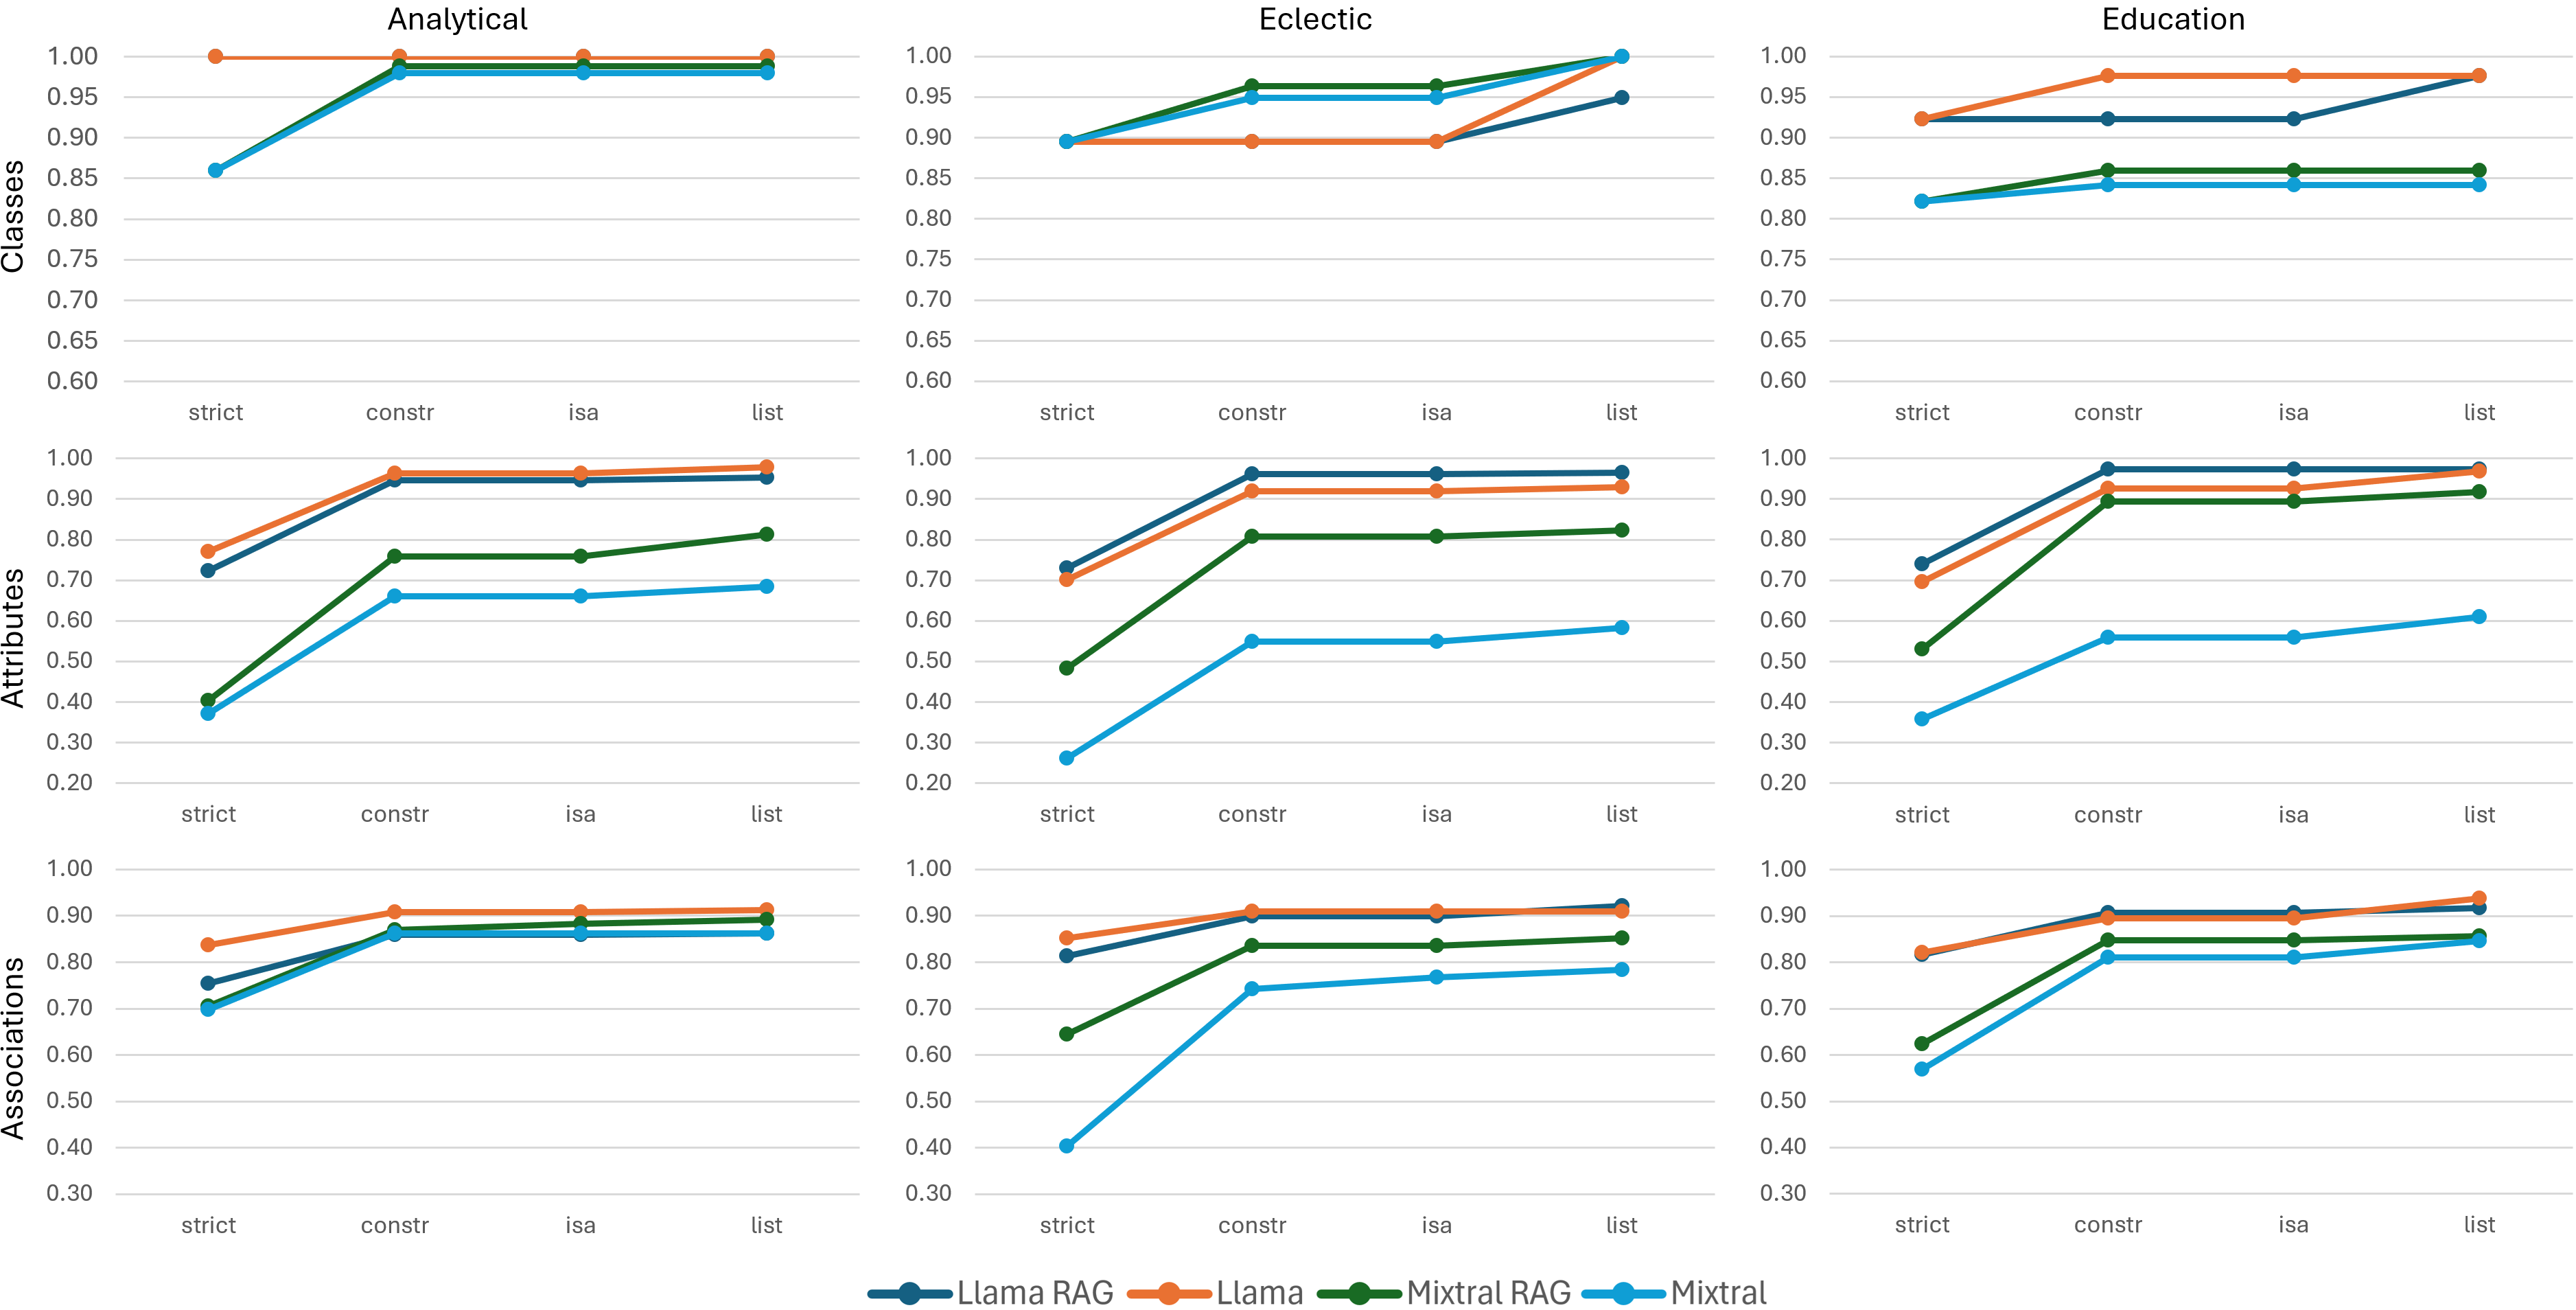
\includegraphics[scale=0.10]{img/evaluation-simple-f1.png}
%    \caption{\centering Average $F_1$ score for the analytical, eclectic, and educational domain descriptions at the four levels of matching strictness}
%    \label{fig:evaluation-simple-f1}
%\end{figure}


\section{User-based evaluation of the application}

In addition to the measurements of the performance of the genererators, we also evaluated how real domain modelers accept an automated domain modeling assistant.

We prepared two domain descriptions, a summary of the main features of the prototype, and three 2-minute video tutorials.

We instructed real users to model the two domains and then asked them to assign a number between 0 (fully disagree) and 4 (fully agree) to express their agreement with five different claims about using our prototype tool.
They also classified themselves as teachers, students, modeling experts, database experts, programmers, or managers (multiple options were allowed).
We received responses from 18 users.

Figure \ref{fig:user-based-evaluation} shows for each type of users the number of responses that picked this type and the average marks received for that type. The last line shows the average of all users.

\begin{figure}[!h]
    %\centering
    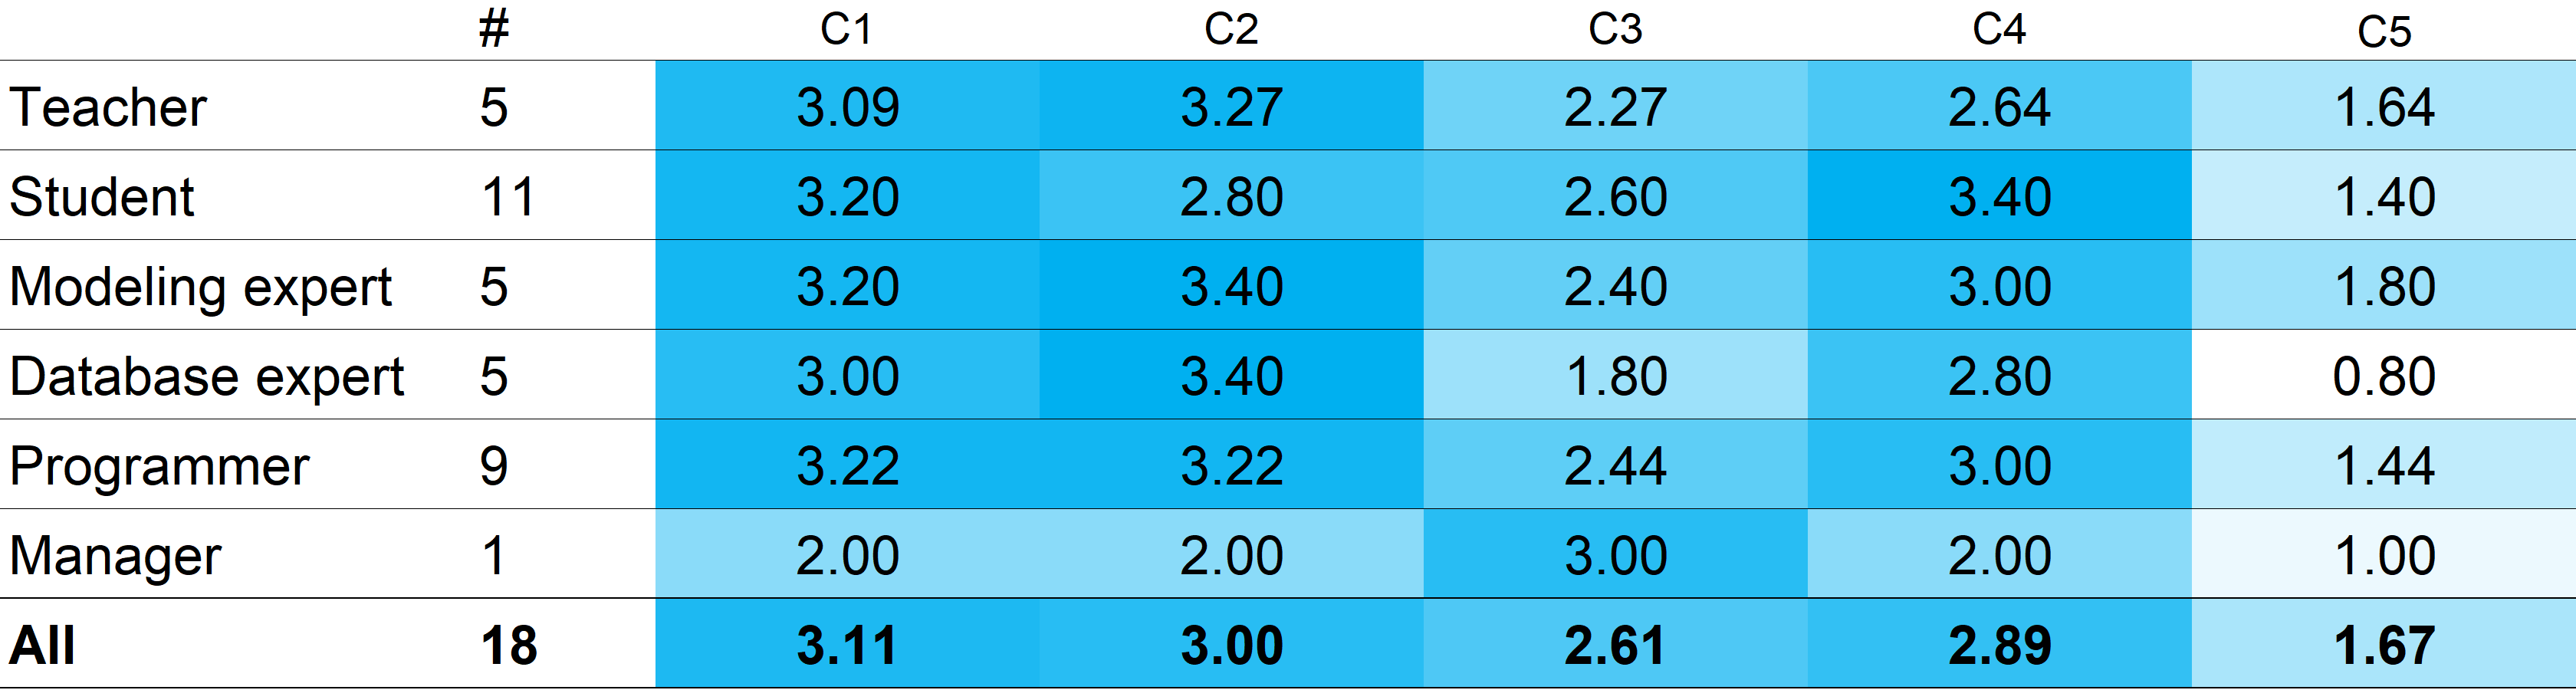
\includegraphics[width=1\linewidth]{img/user-based-evaluation.png} \\
    \scriptsize
\raggedright{C1: Modeling with the assistant is better compared to manual modeling. \\
C2: The assistant is intuitive to use.\\
C3: The assistant suggests appropriate classes, attributes, and associations.\\
C4: The assistant helped me solve the tasks faster compared to manual modeling.\\
C5: I solved all the tasks using only the assistant, and manual modeling was not needed.}
    \caption{Summary of the user-based evaluation. 0=fully disagree, 4=fully agree.}
    \label{fig:user-based-evaluation}
\end{figure}

As we can see, the users agree that using the automated assistant is better than pure manual modeling (C1) and found it intuitive (C2).
The suggestions provided by the tool are subjectively not always appropriate (Q3), which is also supported by our measurements presented in the previous part, and manual modeling is still necessary (Q5).
Despite these imperfections, users claimed that the prototype made them more productive (Q4).
We can find the weakest support in the manager category, but we were able to get only one response in this category, so a further evaluation is necessary.